\documentclass{beamer}
\usetheme{default}
\useoutertheme{infolines}
\usepackage{graphicx}

% logo
\logo{
\includegraphics[height=0.1\textwidth]{./images/rock.png}}

\title{Rock Your Page}
\subtitle{A Chrome Extension Makes Your Webpage More Controlled}
\author{\and{WANG Yue}\and{LUO Xuan}\and{LI Zhi}}
\institute[HKUST]{
    Department of Computer Science \\
    Hong Kong University of Science and Technology \\
}
\date{November 14, 2013}


\begin{document}
\begin{frame}[plain]
    \titlepage
\end{frame}

%%%%%%%%%%%%%%%%%%%%%%%% For Luoxuan: Product Manager %%%%%%%%%%%%%%%%%%%%%%%%
% Motivation
% Overview Features
% Three components
\begin{frame}{Rock Your Page: Features Overview}
Three Components:
\begin{itemize}
    \item Page Sizer: adjust size of contents in web pages based on distance between your face and screen automatically.
    \item Page Rotater: map your 2D web page into 3D scene, multiple pags projection is also supported.
    \item Page Rocker: a small game which let your web page dance with music.
\end{itemize}
\begin{center}
    \begin{figure}
        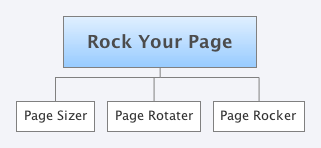
\includegraphics[width=0.4\textwidth]{./images/Rock_Your_Page.png}
        \caption{Overview of Components}
\end{figure}
\end{center}
\end{frame}

\begin{frame}{Rock Your Page: Prototype}
    \begin{center}
        \begin{figure}
            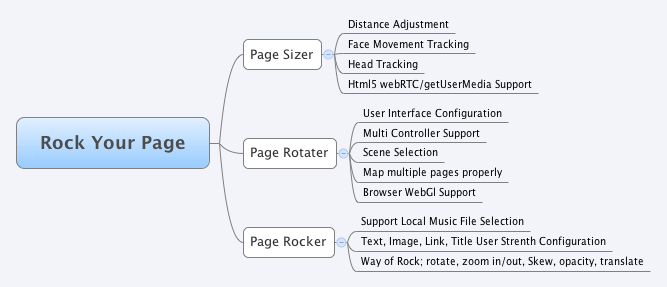
\includegraphics[width=0.8\textwidth]{./images/prototype.png}
            \caption{Prototype Design}
        \end{figure}
    \end{center}
\end{frame}

%%%%%%%%%%%%%%%%%%%%%%% For Wangyue: technical details %%%%%%%%%%%%%%%%%%%%%%%%
%% Functions
%% Technical Details
% chrome extension
\begin{frame}{Technical Overview: Chrome Extension Development}
    \begin{figure}
        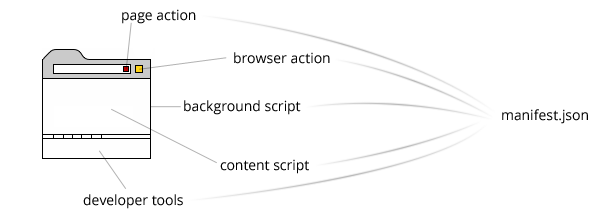
\includegraphics[width=0.8\textwidth]{./images/architecture.png}
        \caption{Architecture of Chrome Extension}
    \end{figure}
\end{frame}

\begin{frame}{Technical Details: Page Sizer}
\begin{center}
    \begin{figure}
        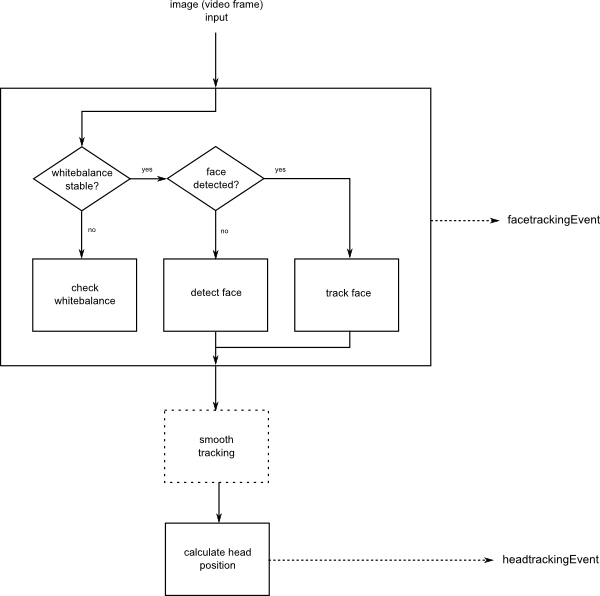
\includegraphics[width=0.6\textwidth]{./images/face_detectin.png}
        \caption{Face Detection in JavaScript}
    \end{figure}
\end{center}
\end{frame}

\begin{frame}{Technical Details: Page Sizer}
\begin{center}
    \begin{figure}
        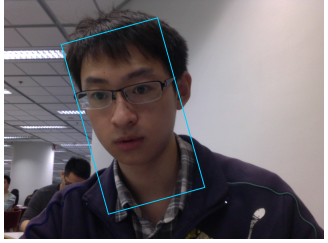
\includegraphics[width=0.25\textwidth]{./images/face_detection_realtime.png}
        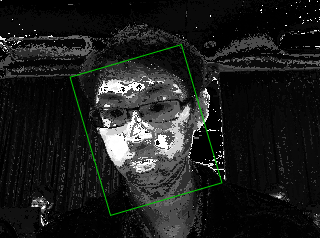
\includegraphics[width=0.25\textwidth]{./images/face_detection_possibility.png}
        \caption{Realtime Face Detection Using Web Camera}
    \end{figure}
\end{center}
Which element in web page shouled be sized?
\begin{itemize}
    \item p,a,h1,h2,h3,h4,h5,h6,code,span,img,pre 
\end{itemize}
How should we detemine the zoom amp?
\begin{equation}
    zoom\_value = (face\_width / video\_width) / (face\_init\_width / video\_init\_width)
\end{equation}
\end{frame}

% Page Rotater
\begin{frame}{Technical Details: Page Rotater}
One single web page mapped into 3D world.
\begin{center}
    \begin{figure}
        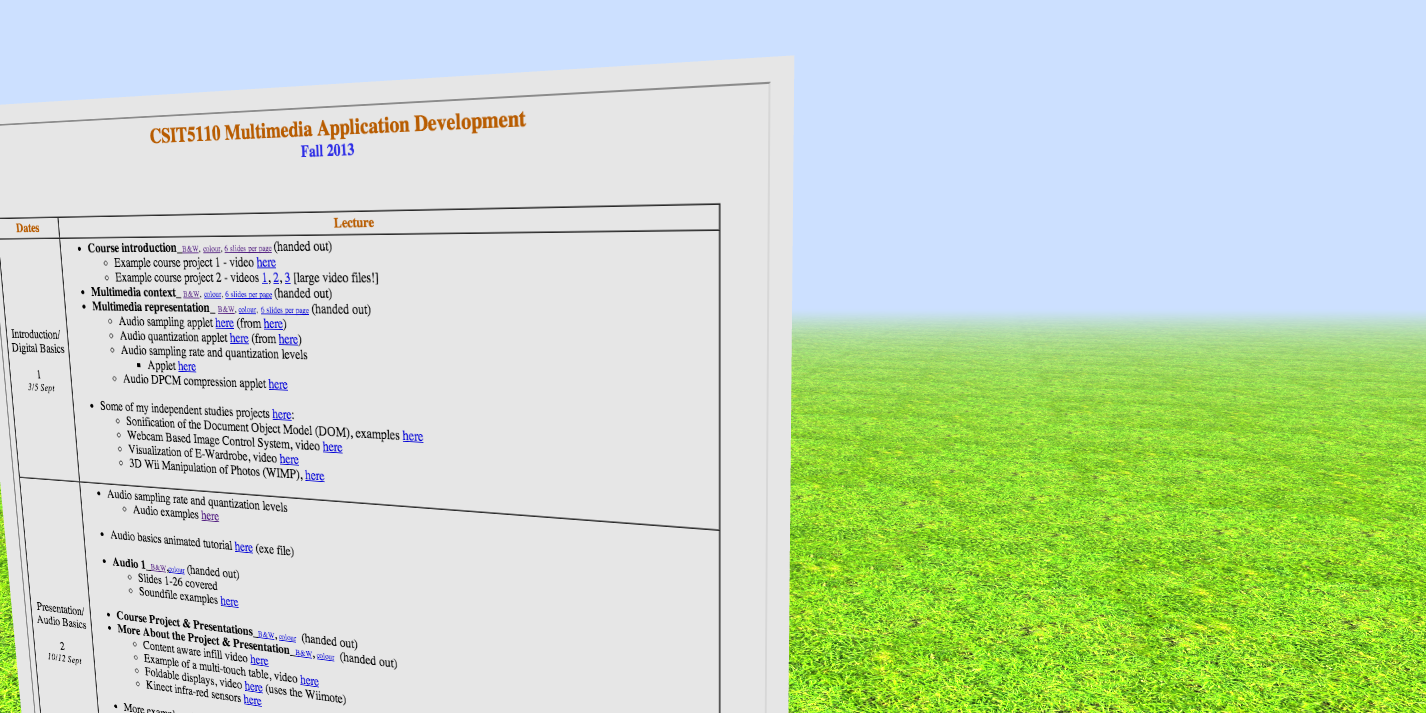
\includegraphics[width=0.8\textwidth]{./images/3d_webpage.png}
        \caption{One single Webpage Mapped to Three-Dimension Scene}
    \end{figure}
\end{center}
\begin{center}
\end{center}
\end{frame}

% multiple web pages
\begin{frame}{Technical Details: Page Rotater}
Map one or several pages into 3D world.
\begin{center}
    \begin{figure}
        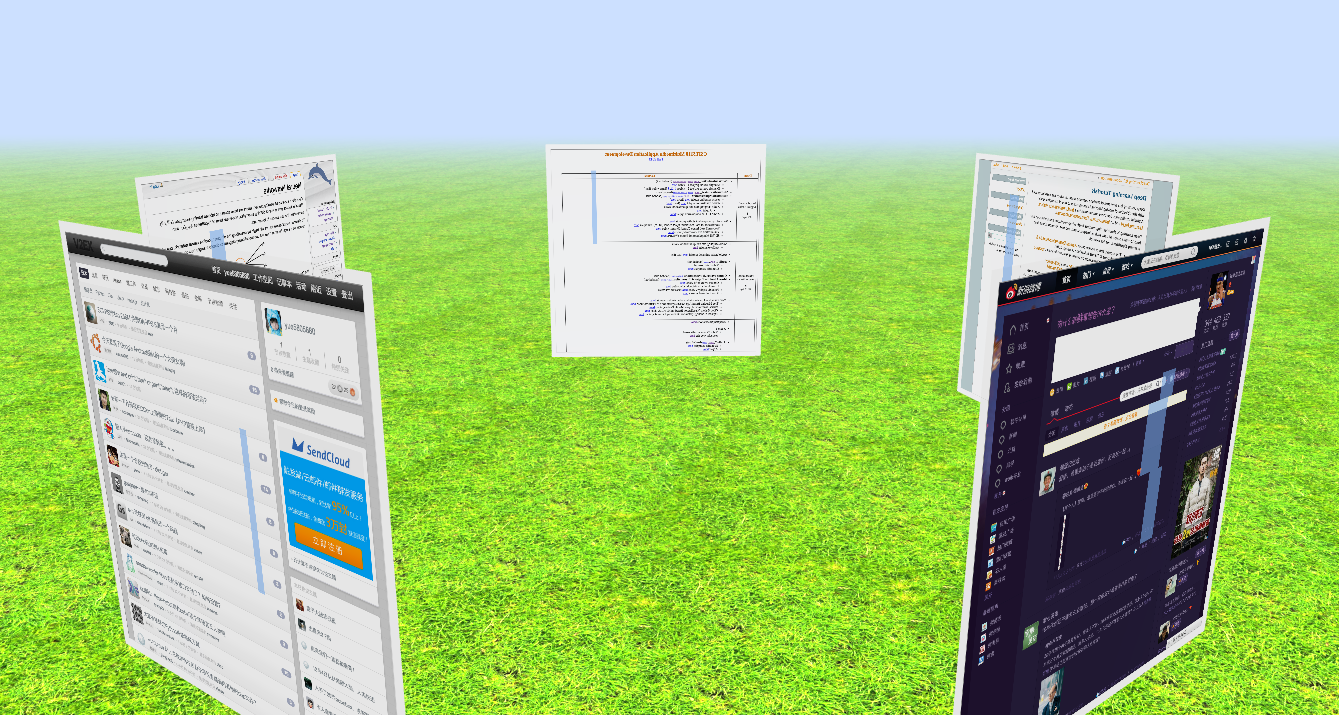
\includegraphics[width=0.8\textwidth]{./images/multi-3d-webpages.png}
        \caption{One single Webpage Mapped to Three-Dimension Scene}
    \end{figure}
\end{center}
\begin{center}
\end{center}
\end{frame}

\begin{frame}{Technical Details: Page Rotater}
How we could combine the current webpage with a 3-D Scene.
\begin{center}
    \begin{figure}
        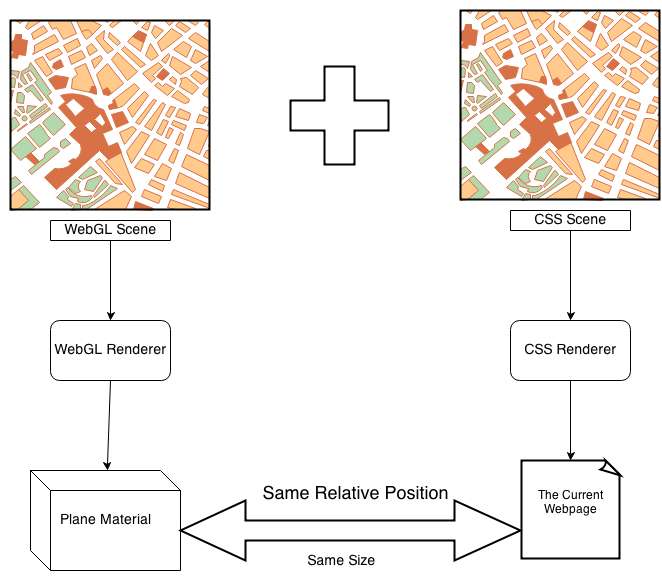
\includegraphics[width=0.5\textwidth]{./images/css3d.png}
        \caption{Map a webpage to a 3D scene}
    \end{figure}
\end{center}
So even in 3D world we can interact with our pages individually without problem.
\end{frame}


\begin{frame}{Technical Details: Page Rotater}
When there n pages, how to set their position and rotation in 3D scene.
\begin{enumerate}
    \item calculate the angle for the ith webpage: $angle = \pi * 2 * i / n$
    \item The position of ith webpage: $Position_{x} = radius * sin(angle)$ and $Position_{z} = radius * cos(angle)$
    \item The rotation of ith webpage: $Vector(0, angle, 0)$
\end{enumerate}
\end{frame}

% rocker technical details
\begin{frame}{Technical Details: Page Rocker}
HTML5 Web Audio Context:
\begin{center}
    \begin{figure}
        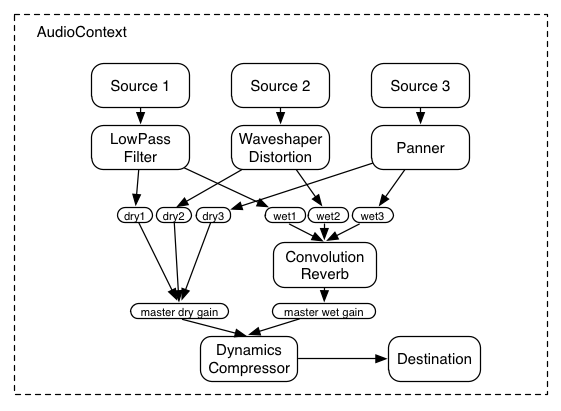
\includegraphics[width=0.7\textwidth]{./images/audiocontext.png}
        \caption{Web Audio Context}
    \end{figure}
\end{center}
\end{frame}

% different ways of rocking
\begin{frame}
Now Four Ways to make page dance with music:
\begin{itemize}
    \item 
\end{itemize}
\end{frame}

% configuraion not included

% development details
%% Team work
%% development env
%% develop tools

%%%%%%%%%%%%%%%%%%%%%%% For LiZhi: Future Work %%%%%%%%%%%%%%%%%%%%%%%%
%% Issues
% Future
\end{document}
